\documentclass[a4paper]{article}

%% Language and font encodings
\usepackage[english]{babel}
\usepackage[utf8x]{inputenc}
\usepackage[T1]{fontenc}

%% Sets page size and margins
\usepackage[a4paper,top=3cm,bottom=2cm,left=3cm,right=3cm,marginparwidth=1.75cm]{geometry}

%% Useful packages
\usepackage{amsmath}
\usepackage{graphicx}
\usepackage[colorinlistoftodos]{todonotes}
\usepackage[colorlinks=true, allcolors=blue]{hyperref}

\title{Algorithms. A Collection of Problems}
\author{Zhengyang Song}

\begin{document}
\maketitle

\section{Longest path in a DAG}

We are given a directed acyclic graph $G$ and two specific vertices $s$ and $t$ in $G$. Each edge in the graph has a length. Design a polynomial time algorithm that finds the longest path from $s$ to $t$. (if there is not path from $s$ to $t$, your algorithm should be able to detect the fact.)

\ \\{\bf Solution:} First do a topology sort in polynomial time. If $t$ is before $s$, return no path. We now only care about the edges between $s$ and $t$, discard all the others. 

Then run a DFS to enumerate the graph.


\section{Monge Matrix}
\[
A[i,j] + A[k,l] \le A[i,l]+A[k,j], \forall i<k\ \text{and}\ j<l
\]
\[\begin{pmatrix}
10 & 9 & 12 & 10\\
11 & 10 & 13 & 10\\
9 & 8 & 0 & 7\\
11 & 10 & 11 & 8
\end{pmatrix}\]
Let $f(i)$ be the column index of the leftmost minimum element of row $i$.
\begin{enumerate}
\item Show that $f(1)\le f(2)\le \dots\le f(m)$.
\item Given an $m\times n$ Monge matrix, design an algorithm that computes $f(1),\dots,f(m)$ in $O(m+n\log m)$ time.
\end{enumerate}
{\bf Solution:}
\begin{enumerate}
\item For $i < j$, we want to prove $f(i) \le f(j)$. Suppose otherwise, we have $f(i) = s > f(j) = t$. Then 
\[
A[i,s] < A[i,t]
\]
\[
A[j,t] \le A[j,s]
\]
\[
A[i,s] + A[j,t] < A[i,t] + A[j,s]
\]
It contradicts with the definition of Monge matrix.
\item We use divide-and-conquer. We first find $f(\lfloor m/2\rfloor)$ in time $O(n)$. Then based on the above conclusion, we can safely drop the bottom left quarter and top right quarter. Do the same operation for the top left quarter and bottom right quarter. Note that this procedure will end in $O(\log m)$ rounds. In each round, the total time cost for all the subtasks are $O(n)$. Furthermore, output all the results will cost time $O(m)$. That leads us to the time complexity of $O(m+ n\log m)$.
\end{enumerate}


\section{}

An interval graph is undirected graph $G=(V,E)$ where vertices correspond to intervals on the real line, where each interval is specified by a leftmost value $v_1$ and a rightmost value $v_2$. Two vertices in $G$ are connected iff the corresponding intervals overlap. Let $G$ be an interval graph whose corresponding intervals are provided. Give a polynomial time algorithm to find a maximum independent set in $G$. You need to prove the correctness of your algorithm. (An independent set in a graph is a subset of vertices such that no two vertices in the subset are joined by an edge.)

\ \\{\bf Solution:} This problem is equivalent to find the maximum set of intervals with no intersection. We can use greedy algorithm. First sort the intervals using the rightmost value as key. Then go through the sorted list, each time we select the interval with the minimal rightmost value that has no intersection with the already selected ones. We show the correctness as follows.

Suppose there is another set of intervals $S'$ that is different from the result of our algorithm $S$. Then after sorting $S'$, we can always find the first interval $i'$ in $S'$ that is different from $i$ in $S$. We simply replace $i'$ with $i$, note that this will not violent the independent property. We can always do this until the last element of $S'$. Thus we have $|S'| \le |S|$


\section{}

Show that finding a min-cost matching with exactly $k$ edges in a bipartite graph $G(U,V;E)$ (with positive edges) can be solved in polynomial time. Note that $|U|$ may not be the same as $|V|$. You can assume that the min-cost perfect matching problem in a bipartite graph can be solved in polynomial time.

\ \\{\bf Solution:} We can turn this into a minimum-cost maximum-flow probelm. Add a source $s$ and a sink $t$, together with a $s'$ and $t'$, where there is an edge with capacity $k$ from $s$ to $s'$, and an edge with capacity 1 from $s'$ to all the vertices in $U$. The same is with $t'$ and $t$. The edges in $E$ are all assigned with a capacity 1. All newly added edges are assigned with a cost 0. Then we just need to compute the minimum-cost maximum-flow of this new graph $G'$, where a polynomial algorithm exists.


\section{Finding the maximum area polygon}

\ \\{\bf Solution:} We can use a dynamic programming method. Suppose the polygon is rooted at 0, then we let $dp[m][i]$ be the maximum area we can get for a $m$-gon with the largest index vertex $i$. 
\[
dp[m][i] = max(\{dp[m-1][j]+area(0, i, j)|j<i\})
\]
Then the answer for root 0 is just
\[
answer = max(\{dp[n][i] | 1\le i\le n\}) 
\]
Then we enumerate all the possible root position (rather than 0) in time $O(n)$. That completes our polynomial algorithm.
\section{Edit distance}

In order to transform one string x to a target string y,we can perform various edit operations. Our goal is,given x and y,to produce a series of edits that change x to y. We may choose from among edit operations:
\begin{itemize}
\item Insert a letter, (e.g., changing 100 to 1001 takes one insertion) 
\item Delete a letter, (e.g., changing 100 to 10 takes one deletion) 
\item Replace a letter by another (e.g., you need do one replacement to change 100 to 000).
\end{itemize}
Design an efficient algorithm that finds a series of edit operations that change x to y and the total number of edits is minimized. 

{\bf Solution:} Denote $dp[i][j]$ as the optimal number of operations to transform $x[:i]$ to $y[:j]$. Then we have
\[
dp[i][j] = dp[i-1][j-1], \text{if } x[i]=y[j]
\]
\[
dp[i][j] = 1+\min(dp[i][j-1], dp[i-1][j], dp[i-1][j-1]), \text{if } x[i]\ne y[j]
\]
\[
dp[i][j] = i, \text{if } j=0
\]
\[
dp[i][j] = j, \text{if } i=0
\]
The answer is just $dp[len(x)][len(y)]$.

\section{Four Russians Speedup}


\section{General machine learning}

\begin{enumerate}
\item In the curve fitting problem on a set of data points, what is the disadvantage of Nearest Neighbors approach compared to Least Squares method?

\ \\{\bf Solution:} Every time we need to start the computation from zero. It is computationally expensive to find the k nearest neighbors when the dataset is very large. Performance depends on the number of dimensions that we have.

On the other hand, it is important how we compute the distance (there may be unrelated features). Also when the dimension is large, the sample data tends to be located at the corner, causing the distance metric meaningless. One solution is to use weighed features to compute the distance. (Credit to Tianqi Zhao) 

\item True/False ``When training a linear regression estimator, 10-fold cross-validation has smaller bias than 5-fold cross-validation''

\ \\{\bf Solution:} Yes. Bias is different from variance. The model we train as a part of the testing procedure, would be as close as possible to the one that we would get if we trained it on the entire dataset.
\end{enumerate}

\section{Maximum Likelihood (ML)}

\begin{enumerate}
\item 
\[
L(\theta) = \theta\cdot 3\theta\cdot (1-3\theta)\cdot (1-3\theta) = 3\theta^2(3\theta-1)^2
\]
\item 
\[ L(\theta) = \frac{1}{3} (3\theta(1-3\theta))^2 \le \frac{1}{3} (\frac{3\theta+1-3\theta}{2})^4 = \frac{1}{48}
\]
where the equation sign is when
\[
3\theta = 1-3\theta \Rightarrow \theta = \frac{1}{6}
\]
\end{enumerate}

\section{Stick Game}
{\bf Solution:} We just maintain a bool array $win[i]$, which means if there are $i$ sticks left, then the next player will win. Then we show how to compute $win[n]$ in polynomail time.

We initialize 
\[
win[0]=false, win[1]=true, win[2]=false, win[3]=true, win[4]=true
\]

Then the recursion is as 
\[
win[i] = true \text{ if } win[i-1] = false \text{ or } win[i-4]=false
\]
\[
win[i] = false \text{ if } win[i-1] = true \text{ and } win[i-4] = true
\]
\section{Mongo Matrix}
\[
A[i,j] + A[k,l] \le A[i,l]+A[k,j], \forall i<k\ \text{and}\ j<l
\]
\[\begin{pmatrix}
10 & 9 & 12 & 10\\
11 & 10 & 13 & 10\\
9 & 8 & 0 & 7\\
11 & 10 & 11 & 8
\end{pmatrix}\]
Let $f(i)$ be the column index of the leftmost minimum element of row $i$.
\begin{enumerate}
\item Show that $f(1)\le f(2)\le \dots\le f(m)$.
\item Given an $m\times n$ Monge matrix, design an algorithm that computes $f(1),\dots,f(m)$ in $O(m+n\log m)$ time.
\end{enumerate}
{\bf Solution:}
\begin{enumerate}
\item For $i < j$, we want to prove $f(i) \le f(j)$. Suppose otherwise, we have $f(i) = s > f(j) = t$. Then 
\[
A[i,s] < A[i,t]
\]
\[
A[j,t] \le A[j,s]
\]
\[
A[i,s] + A[j,t] < A[i,t] + A[j,s]
\]
It contradicts with the definition of Monge matrix.
\item We use divide-and-conquer. We first find $f(\lfloor m/2\rfloor)$ in time $O(n)$. Then besed on the above conclusion, we can safely drop the bottom left quarter and top right quarter. Do the same operation for the top left quarter and bottom right quarter. Note that this procedure will end in $O(\log m)$ rounds. In each round, the total time cost for all the subtasks are $O(n)$. Furthermore, output all the results will cost time $O(m)$. That leads us to the time complexity of $O(m+ n\log m)$.
\end{enumerate}


\section{Unit tasks scheduling}
\section{Coin changing}
\section{Schedule to minimize completion time}
\section{}
\section{}
\section{}
Given an undirected graph $G(V,E)$, a feedback set is a set $X\subset V$ with the property that $G-X$ has no circles. The undirected feedback set problem asks whether $G$ contains a feedback set of size at most $k$. Show that the problem is NP-complete.
\section{Rearrangeable Matrix}

\section{EM}

Explain and prove the convergence of EM algorithm.

\ \\{\bf Solution:} 
\begin{itemize}
\item Expected complete data log likelihood is a lower bound. 
\item EM monotonically increases the observed data log likelihood.
\end{itemize}

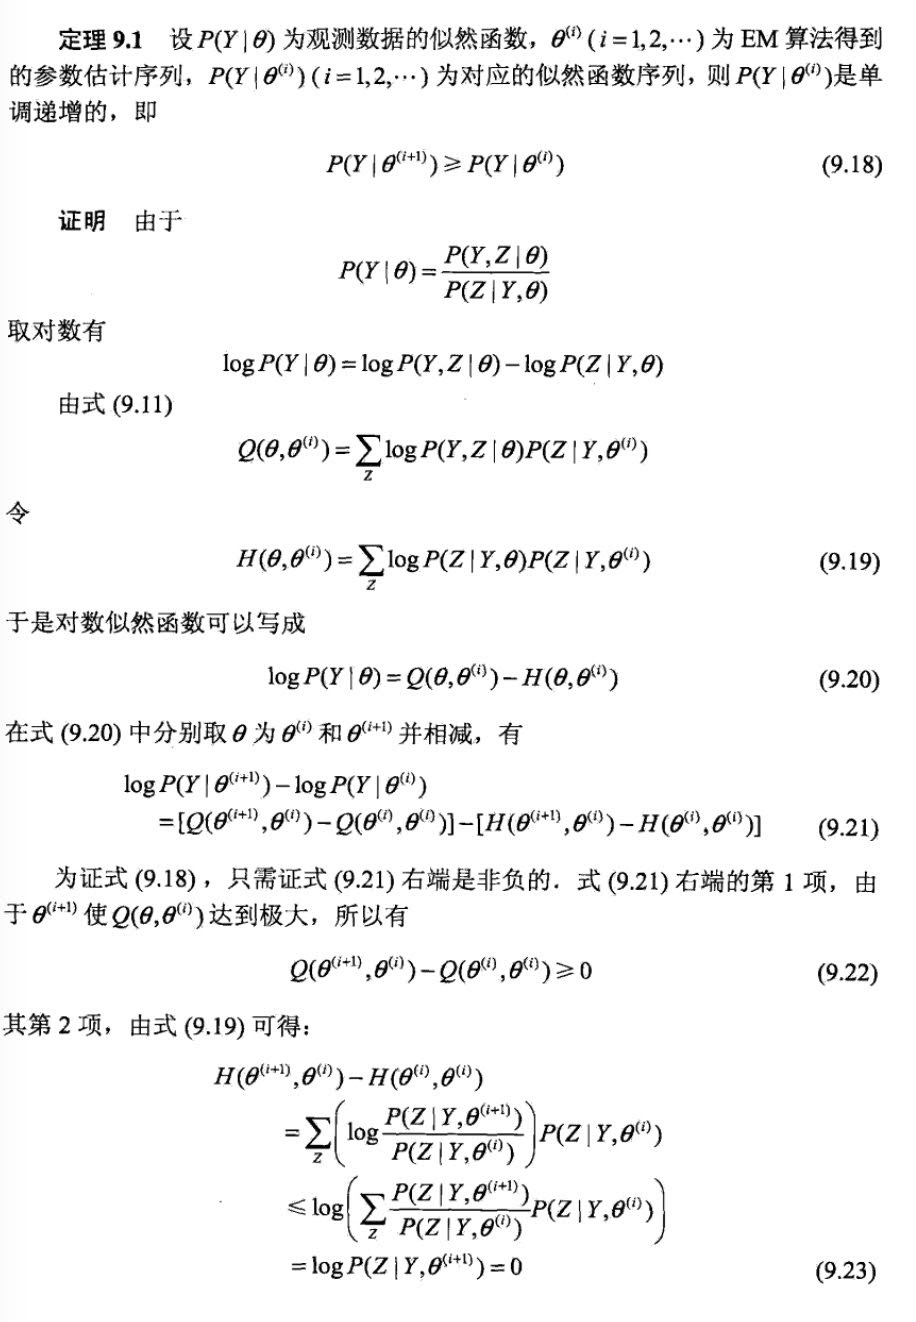
\includegraphics[width=\columnwidth]{19}
\section{Multiple Interval Scheduling}
\section{}

\section{Densest k-Subgraph}

{\bf Solution:} Does $G$ contain a subgraph with exactly $k$ vertices and at least $y$ edges?

First prove it is NP, then prove it is NP-hard.

For an instance $(G, k)$ of  CLIQUE, where $G=(V, E)$, we construct an instance of Dense Subgraph $(G, k, k(k-1)/2)$ in constant time.
\section{Maximum coverage}
{\bf Solution:} Vertex Cover.

Also, we can reducing vertex cover to hitting set.

\section{Polynomial Multiplication}
\[
P(x) = \prod_{i=1}^n(a_ix+b_i)
\]

\section{Longest increasing subsequence}
Design a polynomial time algorithm that finds an longest increasing subsequence in the given sequence $S$.

\ \\{\bf Solution:} We use $dp[i][j]$ to denote the answer of longest increasing subsequence starting from $s[i]$, with the constrain that the first character must be larger than $s[j]$. Suppose the suffix of $s$ is from $1$ to $n$, and $dp[i][0]$ means there is no constrain. So our goal is to get $dp[1][0]$.

The transfer between states are as follows:
\begin{itemize}
\item $dp[n+1][j] = 0$
\item $dp[i][j] = max(1+dp[i+1][i], dp[i+1][j])$, if $s[i] >= s[j]$ and $i <= n$
\item $dp[i][j] = dp[i+1][j]$, if $s[i] < s[j]$ and $i <= n$
\end{itemize}

Note the dp only has $O(n^2)$ different states, that makes our algorithm polynomial.

\section{}
\begin{enumerate}
\item Give a strategy to win this game in a finite number of moves.
\item Show that there is a strategy that guarantees a win if the number of cups $N$ is a power of 2.
\item Show that there is not a strategy that guarantees a win if the number of cups $N$ is not a power of 2.
\end{enumerate} 

\section{}
\section{}
A Hamitonian cycle is a cycle that goes through all vertices exactly once. Prove: Every graph with $n\ge 3$ vertices and minimum degree at least $\lceil n/2 \rceil$ has a Hamitonian cycle.


\section{Catch a car without knowing anything}
\[
p+vt
\]
{\bf Solution:} Since we know the position of the car at time $t$ is $p+vt$, so the problem is that whether we can determine $p$ and $v$ in finite time. That is, if we query position $p_0+v_0t$ at time $t$, and the car is not there, then we can rule out the combination $(p_0, v_0)$. Furthermore, if we check $(p_0, v_0)$ at time $t$, then we can check $(-p_0, v_0)$, $(p_0, -v_0)$, $(-p_0, -v_0)$ at the next three continous time points. So the problem is now turned into whether we can find a way to enumerate $\{(p,v)|p,v\in N\}$ so that a fixed pair $(p_0,v_0)$ can always be encountered in finite time.

Just recall the halting problem and the diagonalization method, i.e., we put all $(p,v)$ onto a two dimensional coordinate, then we enumerate alongside the diagonals: $(0,0)$, $(0,1)$, $(1,0)$, $(0,2)$, $(1,1)$, $(2,0)$, $\dots$ It can be easily shown that this will complete our algorithm.
\section{Turan's bound}

{\bf Solution:} Here we show how to get a indepent set with $|V|\ge\sum\frac{1}{deg(v)+1}$, then $\alpha(G)\ge|V|$.

Everytime, we select the vertex that with the least degree, put it into the indepent set, then delete it and all its neighbors. By doing each step of this, we add 1 to the final result, we distribute this to the $d+1$ nodes, which is 
\[
1 = (d+1)\frac{1}{d+1} \ge \frac{1}{d+1} + \frac{1}{v_1+1} + \frac{1}{v_2+1}+\dots+\frac{1}{v_d+1} 
\]

\section{Traveling salesman in the unit square}
\begin{enumerate}
\item 
\[
|v_1v_2|^2+\dots+|v_{n-1}v_n|^2+|v_nv_1|^2 \le 4
\]
\item {\bf Solution:} Cauchy's Inequality.
\begin{eqnarray*}
&&(|v_1v_2|+\dots+|v_{n-1}v_n|+|v_nv_1|)^2 \\
&\le& (1^2+1^2+\dots+1^2)\cdot (|v_1v_2|^2+\dots+|v_{n-1}v_n|^2+|v_nv_1|^2) \\
&=& n\cdot (|v_1v_2|^2+\dots+|v_{n-1}v_n|^2+|v_nv_1|^2) \\
&\le& n\cdot 4
\end{eqnarray*}
\end{enumerate}
\section{}
\begin{enumerate}
\item {\bf Solution:} BFS
\item {\bf Solution:} BFS
\item 
\end{enumerate}
\section{}
\section{}
Initially, we have $n$ empty bins. In each round, we throw a ball into a uniformly random chosen bin. Let $T$ be number of rounds needed such taht no bin is empty. Show that $E[T]=nH_n$ where $H_n = \sum_{i=1}^n\frac{1}{i}$.

\ \\{\bf Solution:} We denote $E_m$ as the expected number of rounds needed when there are still $m$ bins are left empty.
\[
E_m = \frac{m}{n} (1+E_{m-1}) + \frac{n-m}{n} (1+E_m)
\]
\[
E_0 = 0
\]
Then we have
\[
E_m = E_{m-1} + \frac{n}{m}
\]
\begin{eqnarray*}
E_n &=& E_{n-1} + \frac{n}{n} \\
&=& E_{n-2} + \frac{n}{n-1} + \frac{n}{n}\\
&=& E_0 + \frac{n}{1} + \dots + \frac{n}{n} \\
&=& n H_n
\end{eqnarray*}
\section{}
Show that finding a min-cost matching with exactly $k$ edges in a bipartite graph can be solved in polynomial time.

\ \\{\bf Solution:} We can turn this into a minimum-cost maximum-flow probelm. Add a source $s$ and a sink $t$, together with a $s'$ and $t'$, where there is an edge with capacity $k$ from $s$ to $s'$, and an edge with capacity 1 from $s'$ to all the vertices in $U$. The same is with $t'$ and $t$. The edges in $E$ are all assigned with a capacity 1. All newly added edges are assigned with a cost 0. Then we just need to compute the minimum-cost maximum-flow of this new graph $G'$, where a polynomial algorithm exists.
\section{}
\begin{enumerate}
\item In any bipartite graph, the number of edges in a maximum matching equals the number of vertices in a minimum vertex cover.

\ \\{\bf Solution:} Suppose the set of edges in the maximum matching is $M$, the set of vertices in the minimum vertex cover is $K$. Then we want to prove $|K|\ge |M|$ and $|K|\le |M|$.

$|K|\ge|M|$: No vertex in a vertex cover can cover more than one edge of $M$, that is, the number of vertex cover cannot be less than $|M|$. 

$|K|\le|M|$: Here we will find a vertex cover $K$ with exactly $|M|$ vertices. 

\item In any bipartite graph, the number of vertices in a maximum independent set equals the total number of vertices minus the number of edges in a maximum matching.

\ \\{\bf Solution:} A set of vertices is a vertex cover if and only if its complement is an independent set.
\end{enumerate}
\section{}
\section{}

\bibliographystyle{alpha}
\bibliography{sample}

\end{document}